\documentclass[titlepage,landscape]{seminar}
\usepackage{url}
\usepackage{graphicx}
\usepackage{hyperref}
\usepackage{epstopdf}
\usepackage{slides}

\newcommand{\frack}{\frac{1}{k}}

\begin{document}

\myslide{
  \heading{Association mapping}

  \noindent Na\"ive approach. Regression of phenotype on genotype:
  \[
    y_i = x_{ij}\beta_j + \epsilon_{ij} \quad ,
  \]
  where $y_i$ is the phenotype of individual $i$, $x_{ij}$ is the
  genotype of individual $i$ at locus $j$ (0, 1, 2), and
  $\epsilon_{ij} \sim \mbox{N}(0, \sigma^2)$ is the error.
  \vfill
  {\color{red}\bf PROBLEM}: Individuals may be similar to one another
  because of genetic similarity not reflected in the particular
  markers chosen, e.g., relatedness within a population, population
  structure
}

\myslide{
  \heading{Association mapping}

  \noindent Better approach. Regression of phenotype on genotype with
  a random effect reflecting genetic similarity at markers not
  included in the analysis

  \[
    y_i^{(k)} = x_{ij}\beta_j + \phi^{(k)} + \epsilon_{ij}
  \]

  In general $\phi^{(k)}$ may reflect a general measure of
  relatedness, usually estimated from SNPs.
}

\myslide{
\heading{Warfarin resistance}
\vfill
\begin{center}
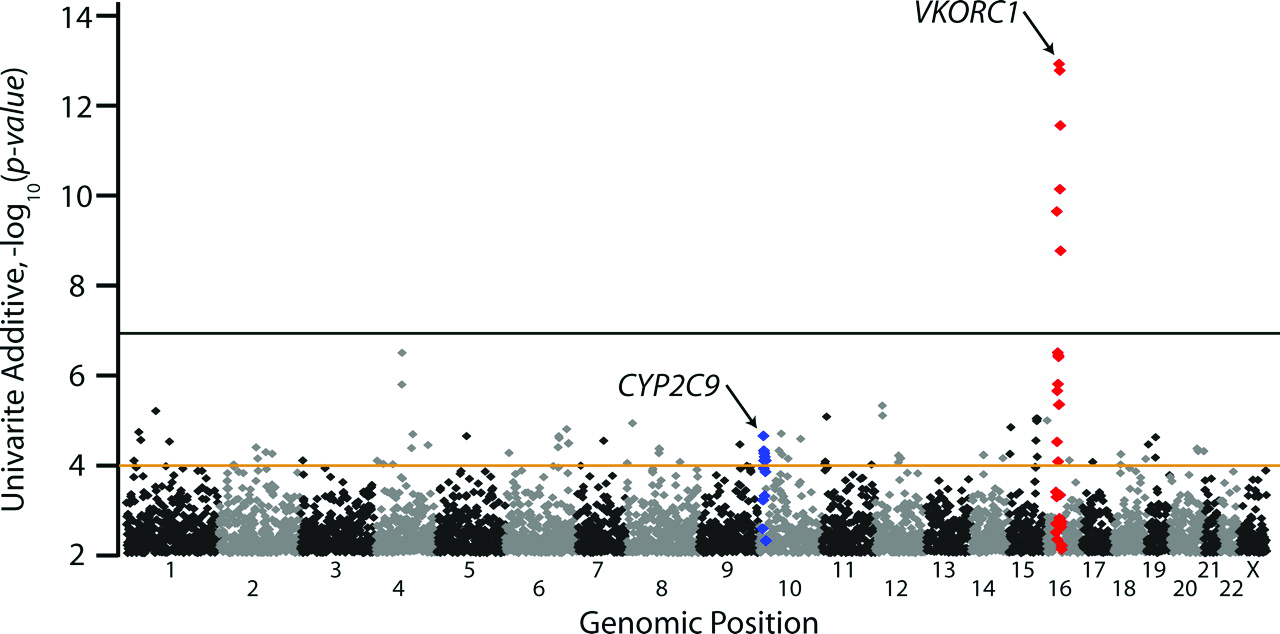
\includegraphics[width=0.9\textwidth]{GWAS-warfarin.eps}
\end{center}
}

\myslide{
  \heading{Two-locus population genetics}
\begin{center}
\begin{tabular}{lcccc}
Gamete    & $A_1B_1$ & $A_1B_2$ & $A_2B_1$ & $A_2B_2$ \\
Frequency & $x_{11}$ & $x_{12}$ & $x_{21}$ & $x_{22}$
\end{tabular}
\end{center}
\vfill
If alleles are arranged randomly into gametes then,
\begin{eqnarray*}
x_{11} &=& p_1p_2 \\
x_{12} &=& p_1q_2 \\
x_{21} &=& q_1p_2 \\
x_{22} &=& q_1q_2 \quad ,
\end{eqnarray*}
where $p_1 = \hbox{freq}(A_1)$ and $p_2 = \hbox{freq}(A_2)$.
}

\myslide{
  \heading{Two-locus population genetics}

  In general,
  \begin{eqnarray*}
    x_{11} &=& p_1p_2 + D \\
    x_{12} &=& p_1q_2 - D \\
    x_{21} &=& q_1p_2 - D \\
    x_{22} &=& q_1q_2 + D \\
    \\
    D &=& x_{11}x_{22} - x_{12}x_{21}
  \end{eqnarray*}

  \vfil
  
  $D$: gametic disequilibrium

  \vfill
}

\myslide{
  \heading{Two-locus population genetics}
\[
\begin{array}{ccccccc}
    &\mu_1            &     &      &     &\mu_2 \\
A_1 &\rightleftharpoons& A_2 &\qquad& B_1 &\rightleftharpoons& B_2
\quad , \\
    &\nu_1            &     &      &     &\nu_2 
\end{array}
\]
\vfill
\begin{eqnarray*}
\frac{\mbox{E}(D^2)}{\mbox{E}(p_1(1-p_1)p_2(1-p_2))}
&\approx& \frac{1}{3 + 4N_er}
\end{eqnarray*}
}

\myslide{
  \heading{Two-locus population genetics}
\begin{center}
\begin{tabular}{c|cccc|cc|c}
\hline\hline
           & \multicolumn{4}{c|}{Gamete frequencies} 
           & \multicolumn{2}{c|}{Allele frequencies} \\
Population & $A_1B_1$ & $A_1B_2$ & $A_2B_1$ & $A_2B_2$ 
           & $p_{i1}$ & $p_{i2}$ & $D$ \\
\hline
1          & 0.24     & 0.36     & 0.16    & 0.24
           & 0.60     & 0.40     & 0.00 \\
2          & 0.14     & 0.56     & 0.06    & 0.24
           & 0.70     & 0.20     & 0.00 \\
Combined   & 0.19     & 0.46     & 0.11    & 0.24
           & 0.65     & 0.30     & -0.005 \\
\hline
\end{tabular}
\end{center}
}

\myslide{
  \heading{Two-locus population genetics}
\begin{eqnarray*}
D_i &=& x_{11,i} - p_{1i}p_{2i} \\
D_t &=& \bar x_{11} - \bar p_1\bar p_2 \\
\bar x_{11} &=& \frac{1}{K} \sum_{k=1}^K x_{11,k} \\
\bar p_1 &=& \frac{1}{K} \sum_{k=1}^K p_{1k} \\
\bar p_2 &=& \frac{1}{K}\sum_{k=1}^K p_{2k}
\end{eqnarray*}
}

\myslide{
  \heading{Two-locus population genetics}
\begin{eqnarray*}
D_t &=& \bar x_{11} - \bar p_1\bar p_2 \\
    &=& \frac{1}{K} \sum_{k=1}^K x_{11,k} - \bar p_1\bar p_2 \\
    &=& \frac{1}{K} \sum_{k=1}^K (p_{1k}p_{2k} + D_k) - \bar p_1\bar p_2 \\
    &=& \frac{1}{K} \sum_{k=1}^K (p_{1k}p_{2k} - \bar p_1\bar p_2) + \bar D \\
    &=& \mbox{Cov}(p_1, p_2) + \bar D \quad ,
\end{eqnarray*}
}

\myslide{
  \heading{Two-locus population genetics}
\begin{eqnarray*}
\mbox{Cov}(p_1, p_2) &=& 0.5(0.6-0.65)(0.4-0.3) + 0.5(0.7-0.65)(0.2-0.3) \\
                     &=& -0.005 \\
\bar x_{11}          &=& (0.65)(0.30) - 0.005 \\
                     &=& 0.19 \\
\bar x_{12}          &=& (0.65)(0.7) + 0.005 \\
                     &=& 0.46 \\
\bar x_{21}          &=& (0.35)(0.30) + 0.005 \\
                     &=& 0.11 \\
\bar x_{22}          &=& (0.35)(0.70) - 0.005 \\
                     &=& 0.24 \quad .
\end{eqnarray*}
}

\end{document}
